\section{Podsystem Windows Forms (9)}

\subsection{Podstawowy interfejs użytkownika (1)} 

    Powtórzyć w Windows Forms zadanie według specyfikacji \ref{okno_dialogowe} ze str.\pageref{okno_dialogowe}.

      [{\bf 1p}]  
	
\subsection{Komponenty dodatkowe (1)} 

    Powtórzyć w Windows Forms zadanie według specyfikacji \ref{common_controls} ze str.\pageref{common_controls}.
	{\em Uwaga!} Komponenty pochodzą z podsystemu Windows Forms.

      [{\bf 1p}]  
	
\subsection{Podsystem {\tt GDI+} (2)} 
    Przedstawiony w skrypcie program rysujący w oknie bieżący czas przerobić na wzór zegarka systemowego
\label{podsystem_gdi}	
      Windows, to znaczy tak, żeby bieżąca godzina była przedstawiana na tarczy zegara analogowego a nie cyfrowego.
      
      Wykorzystać funkcje do rysowania z GDI+. 

      [{\bf 2p}]  
      
\subsection{Własny formant (1)}
      
      Zaimplementować własny komponent {\tt SmoothProgressBar}, który
\label{smooth_progress}	  
      będzie imitować zachowanie standardowego komponentu {\tt ProgressBar} (pasek postępu).
      
      Komponent powinien mieć co najmniej 3 propercje: {\tt Min}, {\tt Max} i {\tt Value}, 
      pozwalające określić odpowiednio minimalną, maksymalną i bieżącą wartość paska postępu.      
      Mając te informacje, {\tt SmoothProgressBar} w zdarzeniu {\tt Paint} powinien rysować gładki 
      (w przeciwieństwie do oryginalnego, który jest złożony z "kafelków")
      pasek postępu o odpowiedniej długości (według zadanych proporcji). 
      
	\begin{figure}
	\begin{center}
	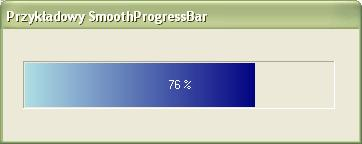
\includegraphics[width=0.6\textwidth]{z6_pb}
	\end{center}
	\caption{Przykładowy {\tt SmoothProgressBar}}
	\end{figure}
      
      [{\bf 1p}]  
	        
\subsection{Pomoc kontekstowa (2)}

    W dowolny sposób przygotować plik pomocy kontekstowej w formacie CHM. 
\label{pomoc_kontekstowa}	
    
    Następnie przykładową aplikację rozszerzyć o obsługę
    pomocy kontekstowej. Należy pokazać, że dla różnych formantów 
    interfejsu użytkownika, przywołanie pomocy kontekstowej przywołuje
    właściwy temat pliku pomocy.
    
    Wskazówki: 
	
	\begin{itemize}
	\item jednym z narzędzni umożliwiających wytworzenie pliku CHM jest darmowy HTML Help Workshop
	\item do wiązania formantów z tematami pomocy można
    użyć bibliotecznego komponentu {\tt HelpProvider} lub jego alternatyw
    w rodzaju 
	
	{\tt http://netpl.blogspot.com/2007/08/con\-text-help-made-easy-reloaded.html}
	\end{itemize}
    
    [{\bf 2p}]  

\subsection{Wykonywanie zadań w tle (1)}

	Zademonstrować w praktyce działanie klasy {\tt BackgroundWorker} oraz jej zdarzenia {\tt ProgressChanged} do delegowania długiego zadania
	do przetwarzania w tle. 
	
	Formalnie - wątek w tle niech testuje jakiś zakres liczb na przykład testem pierwszości. Zakres dobrać tak, aby obliczenia trwały nie krócej niż kilka sekund.
	Postęp obliczeń powinien być raportowany w interfejsie użytkownika za pomocą formantu paska postępu.
	
	Porównać to z zadaniem w tle wykonanym za pomocą standardowego wątka (obiekt {\tt Thread}) który w trakcie obliczeń również aktualizuje pasek	
	postępu obliczeń. Jaka trudność pojawia się w tym drugim podejściu (jest to również odpowiedź na pytanie co wnosi {\tt BackgroundWorker}
	w stosunku do takiego naiwnego podejścia)?

    [{\bf 1p}]  
	
\subsection{Async/await (1)}

	Zaprezentować na niewielkim przykładzie zastosowanie rozszerzeń języka w obszarze programowania asynchronicznego ({\tt async/await}).
	
	Bardziej formalnie - pokazać że w aplikacji okienkowej użycie nieblokującej metody asynchronicznej {\tt HttpClient::ReadStringAsync} 
	do pobrania zawartości z zewnętrznego zasobu sieciowego nie spowoduje zablokowania wątka głównego aplikacji, w którym przetwarzana jest pętla
	obsługi komunikatów. W tej samej aplikacji zademonstrować synchroniczne, blokuące wywołanie metody {\tt WebClient::DownloadString}.
	
    [{\bf 1p}]  

\section{Podsystemy WPF/Metro (4)}

\subsection{Podstawowy interfejs użytkownika (2)} 

    Powtórzyć w WPF zadanie według specyfikacji \ref{okno_dialogowe} ze str.\pageref{okno_dialogowe}.

    [{\bf 2p}]  

\subsection{Komponenty dodatkowe (2)} 

    Powtórzyć w WPF zadanie według specyfikacji \ref{common_controls} ze str.\pageref{common_controls}.
	{\em Uwaga!} Komponenty pochodzą z podsystemu WPF.

    [{\bf 2p}]  
	
